\chapter{Realizzazione del sistema proposto} %\label{1cap:spinta_laterale}
% [titolo ridotto se non ci dovesse stare] {titolo completo}
%

\begin{citazione}
In questo capitolo, le idee e i concetti, definiti precedentemente, saranno realizzati sotto forma di codice funzionante. Attraverso l’implementazione, il sistema prenderà forma, diventando un prodotto software pronto per essere impiegato nella risoluzione dei compiti preposti.
\end{citazione}
\newpage

Come ampiamente esplicitato nei capitoli precedenti, l'obiettivo principale del lavoro svolto è quello di poter analizzare il comportamento di determinati flussi di dati con particolari requisiti di \emph{QoS} in relazione all'utilizzo di diversi protocolli VPN. Vediamo ora nel dettaglio come è stato svolto questo compito.
\subsection{Utilizzo dei protocolli VPN}
Per quanto riguarda l'utilizzo dei protocolli VPN, come è stato presentato nei capitoli precedenti, è stato scelto di utilizzare tre diversi protocolli affinché siano ben chiare le performance ottenibili tramite il loro impiego. I flussi di test precedentemente definiti sono stati scambiati tra client e server i quali sono stati messi in comunicazione tramite l'attivazione di un singolo protocollo VPN per volta in modo da stabilire un canale di comunicazione \emph{cifrato} tra loro. 
Tutti i test eseguiti sono stati portati avanti utilizzando i  protocolli VPN installati \emph{localmente} al sistema realizzato così da evitare l'utilizzo di \emph{container} che avrebbero potuto compromettere i risultati finali dei test.

\section{Sviluppo e integrazione  modulo scansione}
Passiamo ora all'implementazione vera e propria del modulo adibito all'esecuzione delle scansioni dei dispositivi presenti in rete. Come è stato accennato nel capitolo precedente, il presente modulo è stato realizzato impiegando \emph{Python} come linguaggio di programmazione proprio perché offre la possibilità di poter integrare numerose librerie utili allo sviluppo del codice tra cui \emph{Nmap}, \emph{Flask} e \emph{Celery}. Nella figura 5.1 è possibile notare la struttura del progetto realizzato ed i file che lo compongono.
\begin{figure}[h] 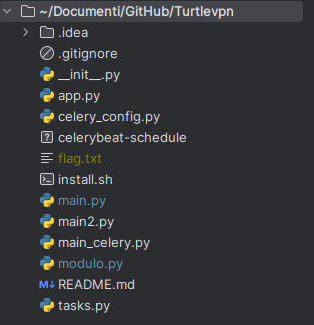
\includegraphics[width=0.5\textwidth] {Tesi magistrale/capitoli/images/file progetto.png}
\centering
\caption{File del progetto.}
\end{figure}

Passiamo ora ad analizzare i principali file che implementano le funzionalità del sistema in questione.

\subsection{modulo.py}
Questo file contiene tutte le scansioni implementate tramite l'utilizzo della libreria \emph{Nmap}. ogni scansione genera un file di output \emph{testuale}, così da poter consultare i risultati anche in un secondo momento dopo la scansione; in particolare sono state implementate diverse scansioni affinché sia possibile cogliere diversi aspetti riguardanti gli host in rete:
\begin{itemize}
    \item \emph{scans (indirizzo)}: elenca i diversi host presenti in rete;
    \item \emph{scans\_time (indirizzo, timer)}: scansione periodica della rete;
    \item \emph{scan\_port (indirizzo, porte)}: scansione di determinate porte;
    \item \emph{scan\_service (indirizzo)}: scansione dei servizi presenti su un indirizzo;
    \item \emph{scan\_os (indirizzo)}: scansione del sistema operativo degli host;
    \item \emph{scan\_vuln (indirizzo)}: scansione delle vulnerabilità degli host.
\end{itemize}

Nella figura 5.2 è riportato un esempio di scansione, in particolare è l'implementazione della scansione \emph{scan\_port}. Per completezza è possibile consultare le altre scansioni all'interno del progetto \emph{GitHub} \cite{pro}.
\begin{figure}[h] 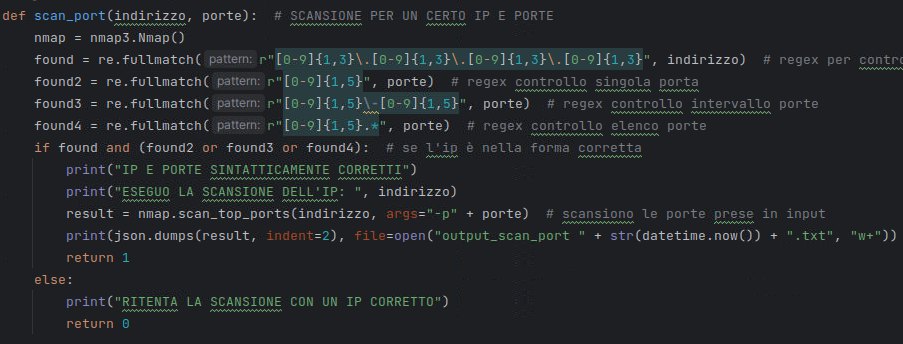
\includegraphics[width=1\textwidth] {Tesi magistrale/capitoli/images/scan.png}
\centering
\caption{Esempio scansione: scan\_port.}
\end{figure}

\subsection{tasks.py}
In questo file sono stati definiti i diversi \emph{task} eseguibili tramite l’impiego di \emph{Celery}, uno scheduler Open Source che permette di programmare l’esecuzione dei task ed anche di eseguirli in modo \emph{asincrono} così da non bloccare l’esecuzione e l’interattività di una pagina web. Nella figura seguente è riportata la definizione di un task per Celery; ovviamente tutti gli altri task sono presenti nel progetto \emph{GitHub} \cite{pro}.
\begin{figure}[h] 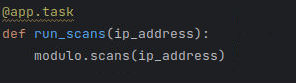
\includegraphics[width=0.5\textwidth] {Tesi magistrale/capitoli/images/task.png}
\centering
\caption{Task per Celery.}
\end{figure}

\subsection{app.py}
In questo file sono state definite le varie \emph{richieste HTTP} in modo da poter utilizzare i task, definiti precedentemente, anche richiamandoli da una possibile pagina web. Le diverse richieste sono state realizzate tramite l’utilizzo di \emph{Flask}, un particolare framework per lo sviluppo web backend in Python.

\begin{figure}[h] 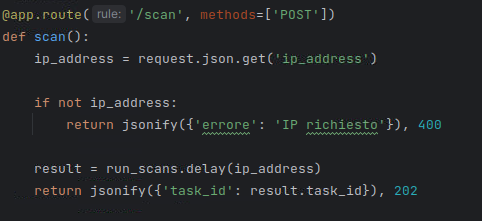
\includegraphics[width=0.6\textwidth] {Tesi magistrale/capitoli/images/app.png}
\centering
\caption{Task per Flask.}
\end{figure}

\section{Sviluppo e integrazione modulo VPN}
In questa sezione è stato sviluppato il modulo inerente all'impiego del protocollo \emph{WireGuard} versione \emph{standard} per fornire agli utenti la possibilità di accedere alle risorse presenti nella rete a cui è connesso il sistema \emph{TurtleVPN} oltre che a fornire la possibilità di poter navigare in rete in modo sicuro.

\subsection{WireGuard e Docker}
A tale scopo è stato utilizzato il gestore di container \emph{Docker} il quale permette di poter gestire in modo agevole i diversi container in cui sono stati istanziati gli applicativi di interesse. In questo caso la versione di Docker utilizzata è la \emph{Compose} \cite{compose} che a differenza della versione standard permette di poter gestire più container allo stesso tempo, di conseguenza offre la possibilità di poter estendere o implementare nuove funzionalità legale all'utilizzo del protocollo WireGuard. Nella figura 5.5 è possibile osservare la configurazione del file \emph{docker-compose.yaml} il quale ha il compito di istanziare i servizi definiti all'interno di esso in base alla configurazione scelta.
\begin{figure}[h] 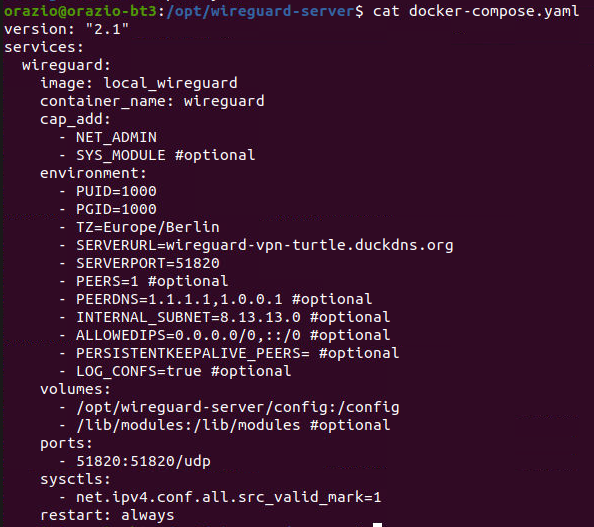
\includegraphics[width=0.6\textwidth] {Tesi magistrale/capitoli/images/wire.png}
\centering
\caption{File docker-compose.yaml.}
\end{figure}

\subsubsection{docker-compose.yaml}
Alcuni dettagli presenti nel file di configurazione:
\begin{itemize}
    \item L'immagine di WireGuard è presente localmente al sistema;
    \item L'indirizzo \emph{reale} del server è stato impostato in modo da fare sempre riferimento all'indirizzo \emph{pubblico} della rete a cui è connesso TurtleVPN in modo che i client possano sempre navigare utilizzando quell'indirizzo. Per raggiungere questo obiettivo è stato impiegato il servizio \emph{Duck DNS} \cite{duck} il quale permette di assegnare ad una stringa l'indirizzo di rete pubblico e di gestire in maniera automatica l'indirizzo di rete fornito dal \emph{provider} anche nel caso in cui cambi dopo un certo lasso di tempo;
    \item La connessione al server WireGuard avviene tramite la porta \emph{51820 UDP};
    \item \emph{8.13.13.0/24} rappresenta la \emph{subnet} assegnata ai dispositivi connessi a TurtleVPN utilizzando un canale sicuro instaurato tramite WireGuard;
\end{itemize}

\subsection{WireGuard client}
Relativamente ai dispositivi client che intendono connettersi al server VPN è necessario che essi eseguano l'\emph{import} del file di configurazione che è stato generato dall'applicativo server WireGuard in esecuzione nel sistema; per i dispositivi mobili è possibile anche effettuare la scansione del \emph{QR-Code} così da poter eseguire l'importazione della configurazione in modo agevole all'interno dell'applicazione client. Nella figura 5.6 è mostrata la configurazione per un client.
\begin{figure}[h] 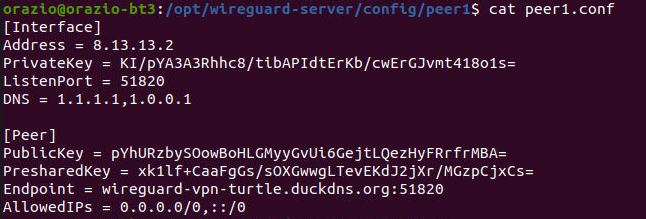
\includegraphics[width=0.7\textwidth] {Tesi magistrale/capitoli/images/confcli.png}
\centering
\caption{Configurazione WireGuard client.}
\end{figure}